\hsection{Loops}%
%
When we are working with sequences of data, we do not just want to perform an action on one specific data element.
We instead often want to apply the actions repetitively to many or even all data elements.
\emph{Loops} allow us to do just that, to perform the same actions multiple times.

In principle, alternatives with \pythonil{if...else} allow us skip certain parts of the code.
In other words, they allow the control flow to jump over them and to continue with what follows after.
Loops are a complementary concept as they allow us to repeat certain parts of the code.
This is basically equivalent to let the control flow jump back to the beginning the the code to be repeated after finishing with its present execution.
Before we delve into this new concept, let us pause a minute and enjoy the significance of what we are going to learn.%
%
\begin{definition}[Structured Programming Theorem]%
The \emph{Structured Program Theorem} states that any computable function can be computed using only three different control flow elements, namely \emph{(1)}~the sequential execution of instructions, \emph{(2)}~the selective execution of instructions~(i.e., alternatives, conditionals), and~\emph{(3)}~the iterative~(repetitive) execution of instructions~(until some condition is met)~\cite{B1964OAFOTMATRPL,BJ1966FDTMALWOTFR,S2011C1GIICS:TBJTAAITSPWP,H1980OFT}.%
\end{definition}%
%
We already learned the first two elements of the control flow.
And now we are going to learn the third one, namely~\emph{loops}.
And after we learned it, we can, basically, perform \emph{any} computation that is possible on today's computers.
Everything that follows after that are devices to make the life of programmers easier.%
%
\pythonIdx{loop}%
%
\hsection{The \texttt{for} Loop Statement}%
%
\pythonIdx{loop!for}%
The most basic such sequence in \python\ may be the \pythonilIdx{for}~loop, which has the following pattern\cite{PSF:P3D:TPT:MCFT}:%
%
\pythonSyntax{syntax/for_loop.py}%
\FloatBarrier%
%
\gitLoadAndExecPython{loops:for_loop_range}{}{loops}{for_loop_range.py}{}%
\listingPythonAndOutput{loops:for_loop_range}{%
An example of using the \pythonilIdx{for} loop over a \pythonilsIdx{range} of integer numbers.}{}%
%
\gitLoadAndExecPython{loops:for_loop_pi_liu_hui}{}{loops}{for_loop_pi_liu_hui.py}{}%
\listingPythonAndOutput{loops:for_loop_pi_liu_hui}{%
A variant of \cref{lst:variables:pi_liu_hui} which uses a \pythonilIdx{for} loop instead of five copies of the same instructions.}{}%
%
The keyword~\pythonilIdx{for} is followed by a loop variable.
Then comes the keyword~\pythonilIdx{in}, the \pythonil{sequence} we want to iterate over, and finally a colon~(\pythonilIdx{:}).
This variable will iteratively take on the values in the \pythonil{sequence}.
The loop body statements is the indented block below the loop header.
It will be executed for each of these values and can access the values via the loop variable.
Each time the body of the loop is executed is called an~\emph{iteration}\pythonIdx{iteration} of the loop.
After the loop, we leave one blank line followed by the code that will be executed after the loop completes.

We already learned about several collection datatypes which could be used as \pythonil{sequence} to iterate over, namely~\pythonilsIdx{list}, \pythonilsIdx{tuple}, \pythonilsIdx{set}, and~\pythonilsIdx{dict}.
However, in its most simple form, the \pythonilIdx{for} loop is applied to a \pythonilIdx{range} of integer numbers.
Ranges are sequences which work basically like slices\pythonIdx{slice} (see \cref{sec:lists,sec:strBasicOperations}).

\pythonil{range(5)} will give us a sequence of integers starting with~0, incrementing in steps of~1, and reaching up to right \emph{before}~5, i.e., the integer range~\intRange{0}{4}.
\pythonil{range(6, 9)} gives the sequence of integers starting with~6, incrementing in steps of~1, and stopping right \emph{before}~9, i.e., the integer range~\intRange{6}{8}.
Finally, \pythonil{range(20, 27, 2)} results in a sequence of integers that begins at~20, increments by~2 in each step, and ends right before~27.
This is the sequence~$(20, 22, 24, 26)$.
\pythonilsIdx{range}, like slices\pythonIdx{slice}, can also have negative increments:
The \pythonil{range(40, 30, -3)} starts with~40 and stops before reaching~30 and decrements by~3 in each step.
This is equivalent to the set~$(40, 37, 34, 31)$.

In program \programUrl{loops:for_loop_range} given as \cref{lst:loops:for_loop_range}, we loop over exactly these ranges.
In this listing, we try to create a dictionary~(see \cref{sec:dictionaries}) where some integer numbers are mapped to their squares.
We use four \pythonilIdx{for}~loops to fill this dictionary with data.
In each of these first four \pythonilIdx{for}~loops, we use \pythonil{i} as the loop variable.

When iterating over the \pythonil{range(5)} in the first loop, \pythonil{i} will hold the value \pythonil{0} in the first iteration~(=~execution of the loop body).
The loop body \pythonil{squares[i] = i * i} will thus effectively be \pythonil{squares[0] = 0} and thus store the value~\pythonil{0} under key~\pythonil{0} into the dictionary \pythonil{squares}.
In the second iteration, \pythonil{i} will hold the value~\pythonil{1}.
Then, the body \pythonil{squares[i] = i * i} will effectively be \pythonil{squares[1] = 1}.
In the third iteration, \pythonil{i} will hold the value~\pythonil{2} and the body will perform \pythonil{squares[2] = 4}.
Next, \pythonil{i = 3} and \pythonil{squares[3] = 9} will be executed and in the laste iteration of the first loop, we store \pythonil{squares[4] = 16}.
With this, the first loop is completed.%
%
\begin{sloppypar}%
In the second loop, which uses \pythonil{range(6, 9)}, \pythonil{i} will take on the values \pythonil{6}, \pythonil{7}, and \pythonil{8}, one by one.
The dictionary \pythonil{squares} will thus be extended with the values \pythonil{squares[6] = 36}, \pythonil{squares[7] = 49}, and \pythonil{squares[8] = 64}.
In the third loop, iterating over \pythonil{range(20, 27, 2)}, the following updates will be performed one by one \pythonil{squares[20] = 400}, \pythonil{squares[22] = 484}, \pythonil{squares[24] = 576}, and \pythonil{squares[26] = 676}.
In the fourth loop, \pythonil{i} takes on the values of the sequence \pythonil{range(40, 30, -3)}, which has the negative step length~\pythonil{-3}.
\pythonil{i}~therefore first becomes~\pythonil{40}, then \pythonil{37} in the second iteration, then \pythonil{34}, and, finally,~\pythonil{31}.
We then \pythonilIdx{print} the dictionary and get the expected output in \cref{exec:loops:for_loop_range}.%
\end{sloppypar}%
%
\bestPractice{underscore}{%
If we do not care about the value of a variable (or parameter), we should name it~\pythonil{_}\pythonIdx{\_}~\cite{PEP635}. %
This information is useful for other programmers as well as static code analysis tools.%
}%
%
At the end of \cref{lst:loops:for_loop_range} we show this special case:
We want to \pythonilIdx{print} \pythonil{"Hello World!"} three times.
Instead of copying the line \pythonil{print("Hello World!")} three times, we put it in a loop iterating over~\pythonil{range(3)}.
However, nowhere in the loop body we care about the value of the loop variable.
We thus simply call it \pythonil{_}\pythonIdx{\_}.

Because of that, everybody reading this code immediately understands that actual value of the counter variable is uninteresting to us.
They will see that we just want to do something three times, that it does not matter which index which iteration has.
If we would not call it that, then another programmer seeing our code~(or a static code analysis tool for that matter) could be confused as to why we do not use the loop variable.
Always remember that \inQuotes{real} code could be much more complicated, and any semantic hint we can include to convey our intentions will be helpful.

With these new tools at hand, we can revisit our program \cref{lst:variables:pi_liu_hui} for approximating~\numberPi\ from back in \cref{sec:approximatePiLiuHui}.
In the original program \programUrl{variables:pi_liu}, we executed the same code five times.
We always doubled the number~\pythonil{e} of edges by doing~\pythonil{e *= 2}.
Then we updated the sidelength~\pythonil{s} of the regular \pythonil{e}\nobreakdashes-gon.
Finally, we printed the approximation of \numberPi\ as \pythonil{e * s / 2}.
Instead of copying the code several times, we can just as well put it inside a loop.
This reduces the lines of code from over~25 to about~10 in program \programUrl{loops:for_loop_pi_liu_hui} given in \cref{lst:loops:for_loop_pi_liu_hui}.
The outputs in \cref{exec:variables:pi_liu_hui,exec:loops:for_loop_pi_liu_hui} are exactly the same.%
%
\FloatBarrier%
\endhsection%
%
\hsection{The \texttt{continue} and \texttt{break} Statements}%
%
\gitLoadAndExecPython{loops:for_loop_continue_break}{}{loops}{for_loop_continue_break.py}{}%
\listingPythonAndOutput{loops:for_loop_continue_break}{%
An example of the \pythonilIdx{continue} and \pythonilIdx{break} statements in a \pythonilIdx{for} loop.}{}%
%
Loops often have complex bodies, maybe containing conditional statements or other loops.
It is not an uncommon situation that, after performing some computations in the body of the loop, we already know that we can continue directly with the next iteration instead of executing the remainder of the loop body.
Sometimes we also find that we can entirely stop with the loop and continue with whatever instructions come after it, even if we did not yet exhaust the sequence over which we are iterating.
The former can be achieved using the keyword \pythonilIdx{continue} and the latter with the \pythonilIdx{break} statement.

An example of both statements is given in \cref{lst:loops:for_loop_continue_break}.
Here, we iterate the variable~\pythonil{i} over the 15~values from~\pythonil{0} to~\pythonil{14}, i.e., over~\pythonil{range(15)}\pythonIdx{range}.
In the loop body, we first create a string~\pythonil{s} with the current value of~\pythonil{i} via the \pgls{fstring} \pythonil{f"i is now \{i\}."}.
The very last instruction of the loop body, \pythonil{print(s)}\pythonIdx{print}, prints this string.

While \pythonil{i} would go from~\pythonil{0} to~\pythonil{14}, we actually want to abort the loop as soon as \pythonil{i} becomes greater than~\pythonil{10}.
We could modify the \pythonilIdx{range} over which we loop, which would be the reasonable thing to do.
Just for fun, we here instead want to use the \pythonilIdx{break} statement.
We therefore wrap it into the conditional \pythonil{if i > 10:}.
If and only if~\pythonil{i > 10}, the \pythonil{break} statement is executed.
The \pythonilIdx{break} will then immediately abort the loop, without even finishing the current iteration.
No further instruction in the loop body is executed and no further iteration is performed.
Instead, the process will continue after the loop, with the line~\pythonil{print("All done.")}.

If \pythonil{i > 10} did not hold, the rest of the loop body is executed.
For the case that $\pythonil{i}\in\intRange{5}{8}$, we now want to directly jump to the next loop iteration.
We do not want to print text and, thus, do not want to invoke the \pythonilIdx{print} in the loop body.
We can achieve this by invoking the \pythonilIdx{continue}~statement.

If \pythonil{5 <= i <= 8} holds, we will invoke \pythonilIdx{continue}.
This means that if \pythonil{i == 5}, the \pythonilIdx{continue}~statement lets the control directly return to the head of the loop.
The loop will set~\pythonil{i = 6}.
Then, the same thing will happen again, and again.
This will continue until~\pythonil{i == 9}.
The condition \pythonil{5 <= i <= 8} is \emph{not} met for all $\pythonil{i}\in\intRange{0}{4}\cup\intRange{9}{15}$.
The next line, namely the \pythonil{print(s)}\pythonIdx{print}, can only be reached in these cases.
Of course, we already know that the loop will terminate anyway as soon as \pythonil{i == 11}.

As a result the program will print the string~\pythonil{s} only for~$\pythonil{i}\in\intRange{0}{4}\cup\{9, 10\}$ before finally outputting~\textil{All done.}.
This can be observed in the program output collected in \cref{exec:loops:for_loop_continue_break}.
With \pythonilIdx{break} and \pythonilIdx{continue}, we now have two tools that can help us to either abort any loop prematurely or to abort the current iteration of the loop prematurely~(and continue with the next one, if any), respectively.%
%
\FloatBarrier%
\endhsection%
%
\hsection{Nesting Loops}%
%
\gitLoadAndExecPython{loops:for_loop_nested_primes}{}{loops}{for_loop_nested_primes.py}{}%
\listingPythonAndOutput{loops:for_loop_nested_primes}{%
Computing a list of all primes from \intRange{2}{200} using nested \pythonilIdx{for} loops.}{}%
%
Like conditional statements, loops can be arbitrarily nested.
The bodies of loops can contain other loops or alternatives.
The branches of alternatives can contain loops as well.
Let us explore this by computing the list of all prime numbers less than~200 in \cref{lst:loops:for_loop_nested_primes}.%
%
\begin{definition}[Prime Number]%
A prime number~$p\in\naturalNumbersO$ is a positive integer~$p>1$, i.e., greater than one, that has no positive integer divisors other than~$1$ and~$p$ itself~\cite{W2024MAWWR:PN,CP2005PNACP,R1994PNACMFF}.%
\end{definition}%
%
In our example program, we want to store all of these prime numbers~$p<200$ in the list\pythonIdx{list} \pythonil{primes}.
We know that \pythonil{2} is a prime number and the only even one, so we directly initialize \pythonil{primes = [2]}, i.e., we set \pythonil{primes} to initially be a list only containing the integer~\pythonil{2}.
This will allow us to later on only consider the odd numbers in the range \intRange{3}{199}.
Just out of interest, we will count the total number of divisions that we need to perform until we have the full list of primes in the variable~\pythonil{n_divisions}.%
%
\begin{sloppypar}%
To find all primes in the integer set~\intRange{2}{199}, we let the loop variable \pythonil{candidate} iterate over~\pythonil{range(3, 200, 2)}\pythonIdx{range}.
This is the sequence of integer numbers starting~\pythonil{3} increasing with step length~\pythonil{2} and stopping right before~\pythonil{200}.
We know that even numbers except~2 are not prime, so this should be OK.
Therefore, \pythonil{candidate} will iteratively become~\pythonil{3}, \pythonil{5}, \pythonil{7}, \dots, and eventually~\pythonil{195}, \pythonil{197}, and \pythonil{199}.%
\end{sloppypar}%
%
For each value of \pythonil{candidate}, we begin with the assumption that it is prime and then try to prove the opposite.
We therefore first set a variable \pythonil{is_prime = True} and then try to find an integer divisor of \pythonil{candidate}.
If we succeed in this, then we set \pythonil{is_prime = False}.
If we cannot find a divisor of \pythonil{candidate}, then \pythonil{is_prime} will remain \pythonil{True}.
In this case, we can add \pythonil{candidate} to the list~\pythonil{primes}.
At least, this is the plan.

We will implement this idea with a nested inner loop.
Since the loop variable \pythonil{candidate} will always be odd, only odd numbers can be potential divisors.
Obviously, only integers greater than or equal to~\pythonil{3} are potential divisors.
We also only need to explore whether a number \pythonil{check} is a divisor of \pythonil{candidate} if it is not bigger than $\sqrt{\pythonil{candidate}}$.
If we had three integer numbers~$a$, $b$, and~$c$ such that $a=b*c$, then it must be that~$c=\frac{a}{b}$.
If~$b>\sqrt{a}$, this means that $c<\frac{a}{\sqrt{a}}$, which means that~$c<\sqrt{a}$.
Viewing this the other way around, since $a=\sqrt{a}*\sqrt{a}$ holds by definition, it would be impossible that $a=b*c$ if both $b>\sqrt{a}$ and $c\geq\sqrt{a}$.
Thus, if $b>\sqrt{a}$ was a divisor of $a$, then there also must be a divisor $c\leq\sqrt{a}$.
And we would discover this divisor with the variable \pythonil{check} before \pythonil{check} reaches~$\sqrt{\pythonil{candidate}}$.

Now, most integer numbers do not have integer square roots.
Since integer divisors cannot have fractions anyway, it is sufficient for us to use $\left\lfloor\sqrt{\pythonil{candidate}}\right\rfloor$.
In \python, such a \inQuotes{truncated} integer square root~$\left\lfloor\sqrt{a}\right\rfloor$ of an integer number~$a$ can be computed using the \pythonilIdx{isqrt} function from the \pythonilIdx{math} module.
We therefore \pythonilIdx{import} this function at the top of our program.%
%
\begin{sloppypar}%
We can therefore iterate a second, inner loop variable \pythonil{check} over \pythonil{range(3, isqrt(candidate) + 1, 2)}\pythonIdx{range}\pythonIdx{isqrt}.
If \pythonil{candidate <= 8}, then this loop will never be executed because no number \pythonil{check} with $3\leq\pythonil{check}<\pythonil{isqrt(candidate)}$ exists.
Then, \pythonil{is_prime} will remain \pythonil{True} and we will append \pythonil{candidate} to \pythonil{primes} further down the outer loop body.
If \pythonil{candidate > 8}, then the loop is actually entered and \pythonil{check} will go from~\pythonil{3} to~$\left\lfloor\sqrt{\pythonil{candidate}}\right\rfloor$.%
\end{sloppypar}%
%
In the body of our inner loop, we try to find out whether \pythonil{check} is an integer divisor of \pythonil{candidate}.
We can do this by computing the remainder of the division~$\pythonil{canddiate}/\pythonil{check}$.
Back in \cref{sec:int:integerArithmetics} we learned the \pgls{modulodiv} operator \expandafter\pythonilIdx{\%}, which does exactly that.
If \pythonil{candidate \% check} is~\pythonil{0}, then we can divide \pythonil{candidate} by \pythonil{check} without remainder.
Then, \pythonil{candidate} is divisible by \pythonil{check} and cannot be a prime number.
We thus can set \pythonil{is_prime = False}.
We can also immediately exit the inner loop using the \pythonilIdx{break} statement.
Once we know that \pythonil{candidate} is not a prime number, we do not need to check further potential divisors.
(Notice that we also count all the \pgls{modulodiv} operations we perform by doing \pythonil{n_divisions += 1} at the beginning of the inner loop.)

After the inner loop, we check whether \pythonil{is_prime} is still \pythonil{True}.
If so, we append \pythonil{candidate} to \pythonil{primes} by invoking the \pythonilIdx{append}\pythonIdx{list!append} method of the list.
Once we have completed the outer loop as well, we print the number~\pythonil{n_divisions} of divisions we have performed, the number~\pythonil{len(primes)}\pythonIdx{len}\pythonIdx{list!len} of prime numbers we have discovered and, finally, the list~\pythonil{primes} of prime numbers itself.
The output in \cref{exec:loops:for_loop_nested_primes} tells us that, after performing 252~divisions, we could identify 46~prime numbers inside~\intRange{2}{199}.
(OK, we ignored or, better, do not know, whether \pythonil{isqrt} performed any divisions {\dots} but let's not be too nit-picky.)%
%
\FloatBarrier%
\endhsection%
%
\hsection{Loops over Sequences}%
\label{sec:loopsOverSequences}%
%
\gitLoadAndExecPython{loops:for_loop_sequence}{}{loops}{for_loop_sequence.py}{}%
\listingPythonAndOutput{loops:for_loop_sequence}{%
An example iterating over the elements in different collection datastructures using \pythonilIdx{for} loops\pythonIdx{loop!for}.}{}%
%
When introducing the \pythonilIdx{for} loop\pythonIdx{for}\pythonIdx{loop!for}, we stated that it iterates over sequences of data.
We learned that \pythonilsIdx{range} are the most basic such sequences.
However, in \cref{sec:collections} we learned about collection datatypes, namely \pythonilsIdx{list}, \pythonilsIdx{tuple}, \pythonilsIdx{set}, and \pythonilsIdx{dict}.
The elements of all of these datatypes can be accessed sequentially, too.
This means that a \pythonilIdx{for} loop can iterate over them as well!

In \cref{lst:loops:for_loop_sequence} we illustrate how this is done:
It works exactly as if we were using \pythonilsIdx{range}.
In the program, we will build a list~\pythonil{txt} with strings that we will later write to the output.

First, we want to iterate over a list\pythonIdx{list}~\pythonil{lst} containing the four integers~\pythonil{[1, 2, 3, 50]}.\pythonIdx{list!iterate over}
This is done by simply writing \pythonil{for i in lst}.
Here, \pythonil{i} is the loop variable and it will step-by-step take on all the values in~\pythonil{lst}, one by one.
In the body of this loop, we invoke \pythonil{txt.append(f"\{i = \}")}.
The \pgls{fstring} will evaluate to \pythonil{"i = 1"} in the first iteration, to \pythonil{"i = 2"} in the second, to \pythonil{"i = 3"} in the third, and to \pythonil{"i = 50"} in the fourth and last iteration of this loop.
These strings are appended to the list \pythonil{txt} via the \pythonilIdx{append}\pythonIdx{list!append} method.

Then we move on and want to iterate over a tuple\pythonIdx{tuple}~\pythonil{tp}, which contains three floating point numbers, namely~\pythonil{(7.6, 9.4, 8.1)}.\pythonIdx{tuple!iterate over}
This works exactly in the same way:
\pythonil{for f in tp} will let the loop variable~\pythonil{f} take on the values \pythonil{7.6}, \pythonil{9.4}, and finally~\pythonil{8.1}.
We again append\pythonIdx{list!append}\pythonIdx{append} their textual representation to the list \pythonil{txt}, this time using the \pgls{fstring} \pythonil{f"\{f = \}"}.

As third example, we create the set\pythonIdx{set}~\pythonil{st} containing the three strings~\pythonil{\{"u", "v", "w"\}}.\pythonIdx{set!iterate over}
We can iterate over the elements this set by, again, simply writing \pythonil{for s in st}.
This lets the loop variable~\pythonil{s} take on the values \pythonil{"w"}, \pythonil{"u"}, and \pythonil{"v"}, \emph{in an arbitrary order}.
Remember that sets in \python\ are unordered (see \cref{bp:setsUnordered}).
This means that if we run the program twice, we may get different results.
Either way, we can iterate over all the values in the set~\pythonil{st}.
We again want to store these values as nicely formatted strings in~\pythonil{txt}.
This time we use the \pgls{fstring} \pythonil{f"s = \{s!r\}"}\pythonIdx{"!r}.
Notice the \pythonil{!r} format specifier\pythonIdx{"!r}:
It will print the \emph{representation} of the string~\pythonil{s}, which basically means to put quotation marks~(and to potentially use \pglspl{escapeSequence}\pythonIdx{str!escaping}\pythonIdx{escaping} for unprintable characters, see \cref{sec:str:escaping}).
Thus, we will add \pythonil{"s = 'v'"}, \pythonil{"s = 'u'"}, and~\pythonil{"s = 'w'"} to \pythonil{txt} (in an arbitrary order).

As fourth and final example, we create a dictionary~\pythonil{dc}\pythonIdx{dict} that maps floating point numbers to Boolean values.
It contains only the two entries, namely~\pythonil{\{1.1: True, 2.5: False\}}.\pythonIdx{dict!iterate over}
Now a dictionary is a bit special:
It maps keys to values.
When working with the whole dictionary datastructure~\pythonil{dc} as a collection, then we can access it in three ways:
%
\begin{enumerate}%
%
\item Iterating over \pythonil{dc} directly lets us view all the keys in the dictionary~\pythonil{dc}. %
This is equivalent to iterating over \pythonil{dc.keys()}\pythonIdx{dict!keys}.%
%
\item Iterating over \pythonil{dc.values()}\pythonIdx{dict!values} lets us access all the values in the dictionary~\pythonil{dc}.%
%
\item Iterating over \pythonil{dc.items()}\pythonIdx{dict!items} lets us access all key-value pairs in the dictionary~\pythonil{dc} as tuples.%
\end{enumerate}%
%
In our example program, we apply all of these methods.
We iterate over the keys in~\pythonil{dc} via \pythonil{for k in dc}, which lets \pythonil{k} take on the values \pythonil{1.1} and \pythonil{2.5}, one after the other.
We iterate over the values in~\pythonil{dc} via \pythonil{for v in dc.values()}, which lets \pythonil{v} take on the values \pythonil{True} and \pythonil{False}, one after the other.%
%
\begin{sloppypar}%
Finally, we iterate over all key-value pairs.
Look closely at this one:
We \emph{could} write \pythonil{for t in dc.items()}, which would let a loop variable~\pythonil{t} take on the tuple values \pythonil{(1.1, True)} and then \pythonil{2.5: False}.
However, back in \cref{sec:tuples}, we learned about tuple unpacking\pythonIdx{tuple!unpacking}\pythonIdx{unpacking}.
So instead, we write \pythonil{for k, v in dc.items()}.
This is basically a shortcut for writing \pythonil{for t in dc.items()} followed by \pythonil{k, v = t}.
It directly unpacks the tuples in the sequence \pythonil{dc.items}.
We thus get pairs of \pythonil{k=1.1}, \pythonil{v=True} and \pythonil{k=2.5}, \pythonil{v=False}.
All of them are again appended to our text list~\pythonil{txt}.%
\end{sloppypar}%
%
After all of these loops, we have ended up with a list~\pythonil{txt} containing~16 strings.
We want to combine all of them to a single string, using \pythonil{", "} as a separator.
We could do this in another loop.
However, \python\ offers us a much more efficient shorthand for this:
The method \pythonilIdx{join}\pythonIdx{str!join} of the class~\pythonilIdx{str}.

For any string~\pythonil{z}, \pythonil{z.join(seq)} accepts a sequence \pythonil{seq} of strings.
It then concatenates all the strings in \pythonil{seq}, placing \pythonil{z} as separator between any two strings.
Thus, invoking \pythonil{", ".join(txt)} produces \textil{i = 1, i = 2, i = 3, i = 50, f = 7.6, ...}.
This text is finally is written to the output via the \pythonilIdx{print} function, giving us the results shown in  \cref{exec:loops:for_loop_sequence}.

\gitLoadAndExecPython{loops:for_loop_sequence_primes}{}{loops}{for_loop_sequence_primes.py}{}%
\listingPythonAndOutput{loops:for_loop_sequence_primes}{%
Computing a list of all primes from \intRange{2}{200} using nested \pythonilIdx{for} loops. %
Compared to \cref{lst:loops:for_loop_nested_primes}, this program is more efficient because it only tests primes as divisors.%
}{}

Let us now use this new ability to iterate over collection datastructures to improve upon our prime number enumeration program \cref{lst:loops:for_loop_nested_primes}.
Back when writing that program, we immediately stored \pythonil{2} as a prime into our list~\pythonil{primes}.
We then only tried the odd numbers less than~200 as potential prime number \pythonils{candidate}.
For each potential prime number \pythonil{candidate}, we tested all (odd) numbers~\pythonil{check} from \pythonil{range(3, isqrt(candidate) + 1, 2)}\pythonIdx{range} as possible divisors.

When thinking about this, we realize that actually, only the prime numbers in this range are interesting.
For example, we do never need to check whether \pythonil{candidate} is divisible by~9, because we will have already checked whether it can be divided by~3.
We also never need to check whether we can divide it by~55, because we will have already checked~5.

But how do we get a sequence that only contains prime numbers?
Well{\dots} actually, we are constructing it already!
\pythonil{primes}~contains all the prime numbers less than~\pythonil{candidate}.

Therefore, in our new and more efficient program \cref{lst:loops:for_loop_sequence_primes}, we replace the head of the inner loop with~\pythonil{for check in primes:}.
As a minor tweak, we leave~2 away from this list at the beginning and instead insert it at the end of the program.
This way, we avoid the useless check whether an odd number \pythonil{candidate} can be divided by~2.

Anyway, the outer loop will step-by-step add prime numbers to \pythonil{primes}.
For each value of the loop variable \pythonil{candidate}, \pythonil{primes} will contain all prime numbers which are smaller than \pythonil{candidate}~(except 2, that is).

We only need to check those values of \pythonil{check} which are less than or equal to \pythonil{isqrt(candidate)}\pythonIdx{isqrt}.
This is because if \pythonil{check} was greater than $\sqrt{\pythonil{candidate}}$, the division would yield a quotient~$q$ less than \pythonil{check}.
If this quotient~$q$ would be a prime number, then this means that we already tested it before.
If it was not a prime number, then it means that~$q$ would be divisible by another number~$r$.
Since $r$ would necessarily be less than~$q$, it would also be less than~\pythonil{check}, and hence, we would have tested it before if it was prime.
If it was not prime, then the argument applies recursively until we eventually hit a prime number.

Therefore, we store this value in a new variable \pythonil{limit} to avoid re-computing it in the inner loop.
The \pythonilIdx{break} statement lets us exit the inner loop as soon as we hit this~\pythonil{limit}.
After the main loop completes, we insert~2 at index~0 into \pythonil{primes}.

The lists of primes that our programs generate in \cref{exec:loops:for_loop_sequence_primes,exec:loops:for_loop_nested_primes} are exactly the same.
However, our new program needs to perform only 224~divisions instead of~252.

Later, in \cref{sec:iteration}, we will learn that loops in \python\ can be applied to the more general concept of~\pythonilsIdx{Iterator}.
We will also see how the \pythonilIdx{for}~keyword can be used to construct sequences via a process called \emph{comprehensions}.%
%
\FloatBarrier%
\endhsection%
%
\hsection{\texttt{enumerate} and Interlude:~Pylint}%
\label{sec:enumOverSequences}%
%
\gitLoadAndExecPython{loops:for_loop_no_enumerate_1}{}{loops}{for_loop_no_enumerate_1.py}{}%
\listingPythonAndOutput{loops:for_loop_no_enumerate_1}{%
Enumerating over the index-value pairs of a list (inefficiently) by using the index as loop variable and directly indexing the container.}{}%
%
\gitLoadAndExecPython{loops:for_loop_no_enumerate_2}{}{loops}{for_loop_no_enumerate_2.py}{}%
\listingPythonAndOutput{loops:for_loop_no_enumerate_2}{%
Enumerating over the index-value pairs of a list (inefficiently) by iterating over the container and manually maintaining the current index in a variable.}{}%
%
Assume that we have a list \pythonil{data} of integer values~\pythonil{v}.
If we want to iterate over all the values~\pythonil{v} in~\pythonil{data}, then \pythonil{for v in data} would do the trick.
However, what if we also want to know the current index~\pythonil{i} for each data element during the iteration?
Then this construct no longer works.

We basically have two choices:
As first option, we can iterate over \pythonil{data} by accessing the elements by their index~\pythonil{i} directly.
In this case, we would use a \pythonilIdx{range} that goes from~\pythonil{0} to \pythonil{len(data) - 1}\pythonIdx{len}\pythonIdx{list!len}.
The head of the loop now looks like this:~\pythonil{for i in range(len(data))}.
The data values~\pythonil{v} are then accessed via~\pythonil{data[i]}.
This is illustrated in \cref{lst:loops:for_loop_no_enumerate_1}.

The drawback of this method is that it will \emph{only} work for \pythonilsIdx{list} and \pythonilsIdx{tuple}.
Among the collection datastructures discussed so far, only \pythonilsIdx{list} and \pythonilsIdx{tuple} are directly indexable.
However, as we have seen, we can iterate over all of them.
Therefore, the second option to achieve our goal would be to just \inQuotes{normally} iterate over the container.
Of course, then we do not know the index of the current element.
Well, nothing can stop us from using an additional integer variable~\pythonil{i} and maintain its proper value by ourselves.
We would initialize it as \pythonil{i: int = 0} before the loop.
We would then increment it as~\pythonil{i += 1} at the bottom of the loop body.
Of course, \pythonil{i += 1} is equivalent to \pythonil{i = i + 1}\pythonIdx{+=}\pythonIdx{+}.
This would work with all collection classes.
This is illustrated in \cref{lst:loops:for_loop_no_enumerate_2}.

Both options are a bit iffy, as they introduce more and less readable additional code.
There is a third option, though.
And because I advocate using static code analysis tools, I let another such tool discover this option for us.%
%
\begin{figure}%
\centering%
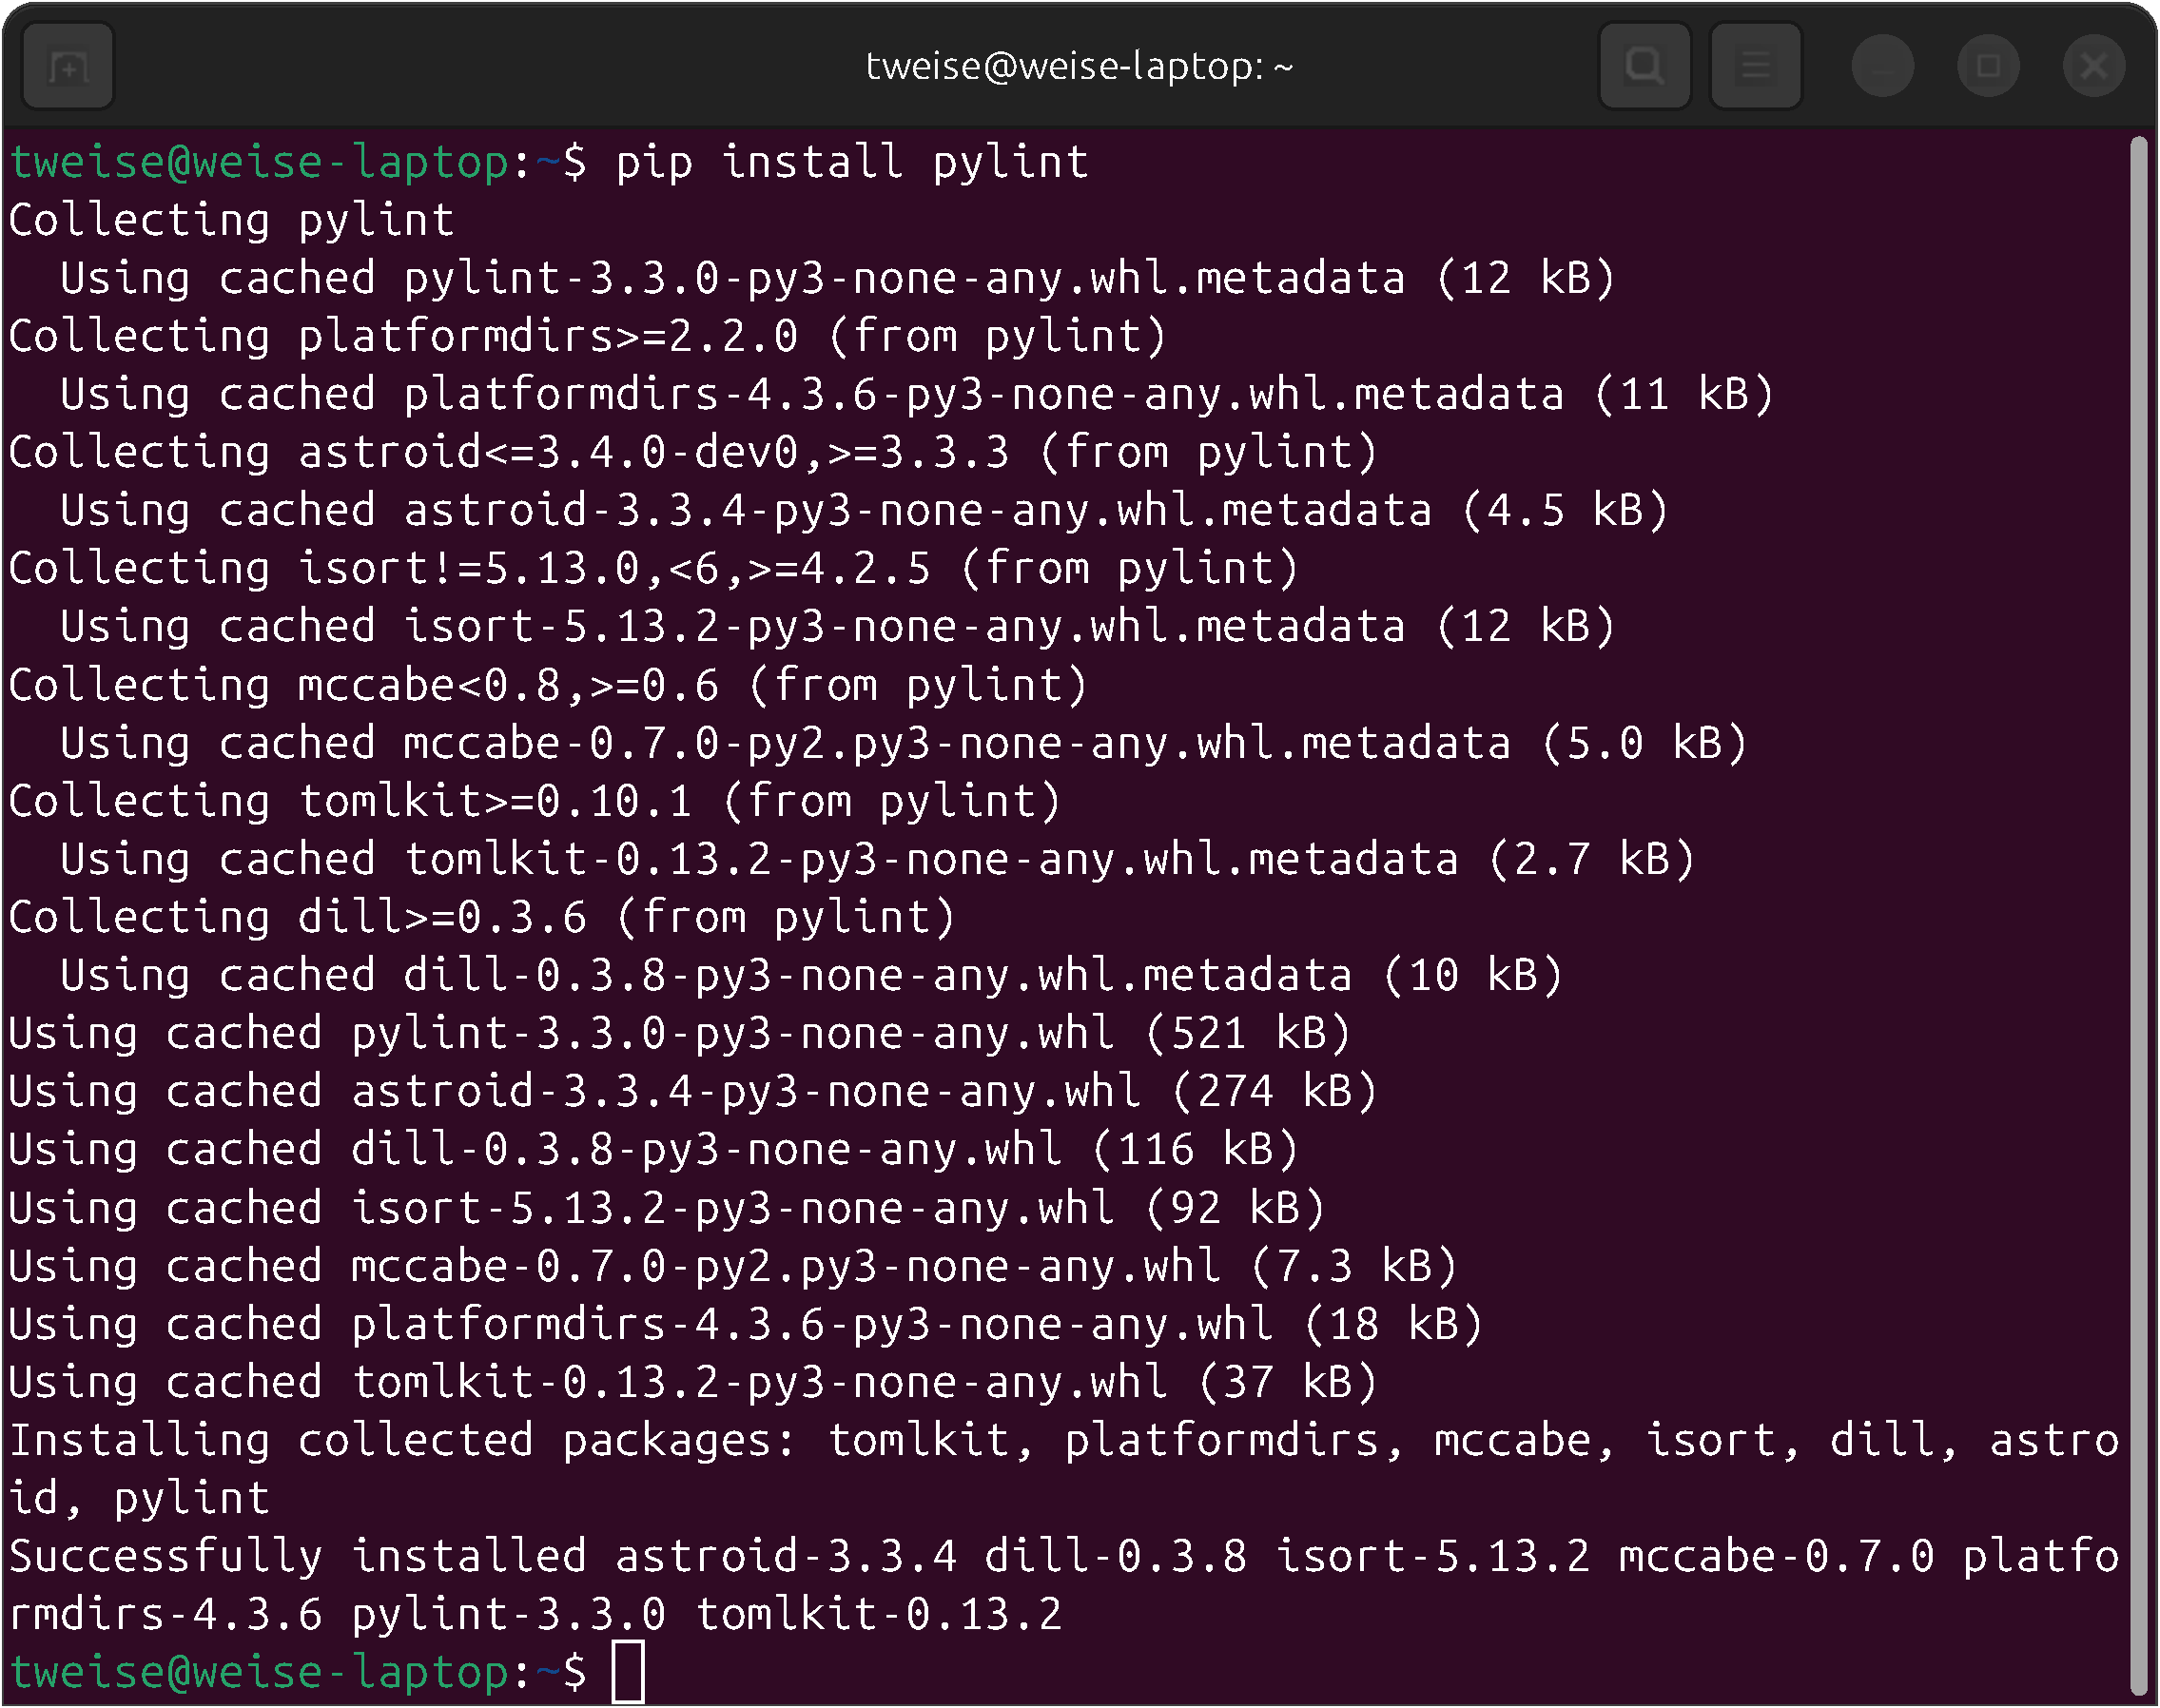
\includegraphics[width=0.7\linewidth]{\currentDir/pipInstallPylint}%
\caption{Installing \pylint\ in a \ubuntu\ \pgls{terminal} via \pip~(see \cref{sec:pipAndVenv} for a discussion of how packages can be installed).}%
\label{fig:pipInstallPylint}%
\end{figure}%
%
\usefulTool{pylint}{%
\pylint\ is a \python\ \pgls{linter} that analyzes code for style, potential errors, and possible improvements~\cite{PC2024PL}. %
It can be installed via \bashil{pip install pylint} as shown in \cref{fig:pipInstallPylint} on \cpageref{fig:pipInstallPylint}. %
You can then apply \pylint\ using the command \bashil{pylint fileToScan.py}. %
We provide a script for using \pylint\ with a reasonable default configuration in \cref{lst:bash:pylint} on \cpageref{lst:bash:pylint}.%
}%
%
\gitExec{exec:loops:for_loop_no_enumerate_1:ruff}{\programmingWithPythonCodeRepo}{.}{_scripts_/ruff.sh loops for_loop_no_enumerate_1.py}%
\gitExec{exec:loops:for_loop_no_enumerate_2:ruff}{\programmingWithPythonCodeRepo}{.}{_scripts_/ruff.sh loops for_loop_no_enumerate_2.py}%
%
\gitExec{exec:loops:for_loop_no_enumerate_1:pylint}{\programmingWithPythonCodeRepo}{.}{_scripts_/pylint.sh loops for_loop_no_enumerate_1.py}%
\gitExec{exec:loops:for_loop_no_enumerate_2:pylint}{\programmingWithPythonCodeRepo}{.}{_scripts_/pylint.sh loops for_loop_no_enumerate_2.py}%
%
\listingToolOutput{loops:for_loop_no_enumerate_1:pylint}{%
The results of static code analysis using the \pylint\ \pgls{linter} for the program \programUrl{loops:for_loop_no_enumerate_1} given in \cref{lst:loops:for_loop_no_enumerate_1}.}%
%
\listingToolOutput{loops:for_loop_no_enumerate_1:ruff}{%
The results of static code analysis using the \ruff\ \pgls{linter} for the program \programUrl{loops:for_loop_no_enumerate_1} given in \cref{lst:loops:for_loop_no_enumerate_1}.}%
%
\listingToolOutput{loops:for_loop_no_enumerate_2:pylint}{%
The results of static code analysis using the \pylint\ \pgls{linter} for the program \programUrl{loops:for_loop_no_enumerate_2} given in \cref{lst:loops:for_loop_no_enumerate_2}.}%
%
\listingToolOutput{loops:for_loop_no_enumerate_2:ruff}{%
The results of static code analysis using the \ruff\ \pgls{linter} for the program \programUrl{loops:for_loop_no_enumerate_2} given in \cref{lst:loops:for_loop_no_enumerate_2}.}%
%
\gitLoadAndExecPython{loops:for_loop_enumerate}{}{loops}{for_loop_enumerate.py}{}%
\listingPythonAndOutput{loops:for_loop_enumerate}{%
Enumerating over the index-value pairs of a list using the \pythonilIdx{enumerate} function.}{}%
%
We first install \pylint~cite{PC2024PL}.
We therefore open a \pgls{terminal} by either pressing \ubuntuTerminal\ under \ubuntu\ \linux\ or \ubuntuTerminal\ or under \microsoftWindows\ via \windowsTerminal.
As sketched in \cref{fig:pipInstallPylint}, we then type in \bashil{pip install pylint}\pythonIdx{pip} and hit \keys{\return}.~(Normally, we would do that in a \pgls{virtualEnvironment}, which we discuss later in \cref{sec:pipAndVenv}.)
Anyway, \pylint\ gets installed.

We can apply it a file \textil{fileToScan.py} by typing \bashil{pylint fileToScan.py} in a \pgls{terminal}~(\textil{fileToScan.py} can also be a directory).
Like with \ruff, in the context of this book, we will disable some \pgls{linter} rules for \pylint, too.
This can be done by adding the parameter \textil{--disable=...} with the rules to be deactivated.
The list of rules that \pylint\ applies when analyzing a file can be found at~\cite{PC2024PL}.%
%
\begin{sloppypar}%
Let us now apply both our new \pgls{linter} \pylint\ as well as \ruff, which we ave already used, to the two ideas for enumerating over the data and indices of collections.
We first analyze \programUrl{loops:for_loop_no_enumerate_1}, the program where we let the index variable iterate and use it to access the data elements.
In \cref{exec:loops:for_loop_no_enumerate_1:pylint}, \pylint\ suggest that we should iterate over the list \pythonil{data} using the \pythonilIdx{enumerate} function, whereas \ruff, at the time of this writing, has no issue with this approach~(see \cref{exec:loops:for_loop_no_enumerate_1:ruff}).
Now we analyze \programUrl{loops:for_loop_no_enumerate_2}, where we iterate over the elements of the container and manually maintain an index variable~\pythonil{i}.
Interestingly, this time \ruff\ suggests us to~\inQuotes{Use \inSQuotes{\pythonil{enumerate()}} for index variable \inSQuotes{\pythonil{i}} in \inSQuotes{\pythonil{for}} loop}, as shown in \cref{exec:loops:for_loop_no_enumerate_2:ruff}.
\pylint, on the other hand, does not discover any problem with \programUrl{loops:for_loop_no_enumerate_2}.%
\end{sloppypar}%
%
Our two \pglspl{linter} have discovered the same issue, just with different programs.
They independently propose using a function called \pythonilIdx{enumerate} to solve the problem of iterating over collections and knowing the index of the current element.
But what is \pythonilIdx{enumerate}?

\pythonilIdx{enumerate} accepts a collection as parameter and creates a sequence of index-value tuples~\cite{PEP279}.
We can unpack such tuples while iterating over this sequence~(see \cref{lst:loops:for_loop_sequence}).
Therefore, when using \pythonilIdx{enumerate}, we can change the head of our loop to the form \pythonil{for i, v in enumerate(data)}.
Notice that the index~\pythonil{i} comes first and the value~\pythonil{v} comes second in this unpacked-tuple-based enumeration.
This is implemented in program \programUrl{loops:for_loop_enumerate} given as \cref{lst:loops:for_loop_enumerate}.
And it would work exactly the same, regardless whether \pythonil{data} was a \pythonilIdx{list}, \pythonilIdx{set}, \pythonilIdx{tuple}, or \pythonilIdx{dict}ionary.

We also confirmed \cref{bp:manyCodeAnalysisTools}:
It makes sense to use several different tools for static code analysis.
Each tool has its own strengths.
Some, like \mypy, can discover problems with typing.
Others, like \ruff\ and \pylint, can make suggestions on how to improve our code.
But even if two tools have the same \inQuotes{area of expertice,} they may still discover different issues.
Had we implemented \programUrl{loops:for_loop_no_enumerate_1} and only used \ruff, at least at the time of this writing, we would not have found that we could use \pythonilIdx{enumerate} to solve the problem more efficiently.
Vice versa, if our solution idea had been \programUrl{loops:for_loop_no_enumerate_2} and only used \pylint, then at the time of this writing, we, too, would not have arrived at the more efficient version \programUrl{loops:for_loop_enumerate.py}.
Thus, indeed, it is important to understand and use the tools that surround our programming language.
And not just one.
Keep learning and adding new tools to your tool belt.%
%
\FloatBarrier%
\endhsection%
%
\hsection{The \texttt{while} Loop}%
\label{sec:whileLoop}%
%
\begin{figure}%
\centering%
\tightbox{
\includegraphics[width=0.5\linewidth]{\currentDir/heronOfAlexandria}}%
\caption{Heron of Alexandria. %
Codex of Saint Gregory Nazianzenos. Greek manuscript of the ninth century~\pgls{CE}. %
Public Domain. %
Source:~\cite{GR:TAGWITWFST}.%
}%
\label{fig:heronOfAlexandria}%
\end{figure}%
%
Old clay tablets show that the Babylonians were able to approximate~$\sqrt{2}$ maybe as far back as 4000~years ago~\cite{FR1998SRAIOBMY7IC,S2011NA:NA}.
The mathematician Hero(n) of Alexandria lived in the first century~\pgls{CE}.
He specified an abstract algorithm for computing the square root of numbers which, today, is known as Heron's Method~\cite{S2011NA:NA,K2009BMOCTSRJBOFTAOCC}.
This famous researcher, illustrated in \cref{fig:heronOfAlexandria}, was also a famous engineer who invented a steam engine~\cite{GR:TAGWITWFST} and a formula for the computation of the area of a triangle~\cite{L2020RWECSSKAFPA}.

Let's say that we want to find the square root~$\sqrt{a}$ of a given~$a$.
Then, this algorithm starts with a guess~$x_0$, let's say~$x_0=1$.
In each iteration, it will compute a new guess~$x_{i+1}$ based on the current approximation~$x_i$ as follows~\cite{S2011NA:NA,K2009BMOCTSRJBOFTAOCC}:%
%
\begin{equation}%
x_{i+1}=\frac{1}{2}\left(x_i+\frac{a}{x_i}\right)%
\label{eq:heronGuessUpdate}%
\end{equation}%
%
We can roughly imagine that the algorithm works as follows:
If $x_i$ was too big, i.e., $x_i>\sqrt{a}$, then~$\frac{a}{x_i}<\sqrt{a}<x_i$.
If $x_i$ was too small, i.e., $x_i<\sqrt{a}$, then $\frac{a}{x_i}>\sqrt{a}>x_i$.
By computing the average of~$x_i$ and~$\frac{a}{x_i}$ as the next guess, we hope to approach~$\sqrt{a}$.
If $x_i=\sqrt{a}$, then $\frac{a}{x_i}=\sqrt{a}$ by definition and~$x_{i+1}=x_i$.
Showing that this actually works and that the error gets smaller over time is more complicated~\cite{S2011NA:NA}.
But luckily, we do not need to do that here.
Let's simply trust the two thousand year old genius Heron.

If we want to implement this algorithm, we will naturally need a loop of some sort.
Clearly, we perform the same computation multiple times.
We will evaluate \cref{eq:heronGuessUpdate} again and again.
However, a \pythonil{for}~loop will not do:
We do not know in advance the number of steps that we will need until~$x_i = x_{i+1}$.
Of course, we could try to pick a very very huge number and then \pythonil{break} the loop when the guesses converge {\dots} but that is just ugly.
The \pythonilIdx{while} comes to rescue\cite{PSF:P3D:TPT:MCFT}:%
%
\pythonSyntax{syntax/while_loop.py}%
\FloatBarrier%
%
\gitLoadAndExecPython{loops:while_loop_sqrt}{}{loops}{while_loop_sqrt.py}{}%
\listingPythonAndOutput{loops:while_loop_sqrt}{%
We compute the square root of a number using Heron's Method~\cite{S2011NA:NA,K2009BMOCTSRJBOFTAOCC} implemented as py \pythonilIdx{while} loop.}{}%
%
Like the \pythonil{for}~loop, the \pythonilIdx{while}~loop has a head and a body.
The head consists of a \pythonil{while}, followed by a loop condition \pythonil{booleanExpression} and a colon~\pythonil{:}.
The loop body is again just a code block indented with four spaces.
Every time \emph{before} the loop body is executed, the loop condition \pythonil{booleanExpression} is evaluated.
If and only if it yields~\pythonil{True}, the loop body is executed.
Only in this case, the next iteration begins by again checking the loop condition, and so on.
If the loop condition does not yield~\pythonil{True}, the loop is immediately terminated.
In other words, the body of the loop is executed as long as a Boolean expression in the head of the loop evaluates to~\pythonilIdx{True}.

We now use this new construct to implement Heron's Method as program \programUrl{loops:while_loop_sqrt} in \cref{lst:loops:while_loop_sqrt} and use it to compute the square roots of~0.5, 2, and~3.

We begin the program with an outer \pythonil{for} loop that iterates a variable~\pythonil{number} over the \pythonil{float} values \pythonil{0.5}, \pythonil{2.0}, and~\pythonil{3.0}.
We want to apply the algorithm to each of these values.
We use two variables~\pythonil{guess} and \pythonil{old_guess}.
\pythonil{guess} will be the current guess of what $\sqrt{\pythonil{number}}$ could be.
\pythonil{old_guess} will be the previous approximation, which we need to remember in order to decide when to stop.

We initialize \pythonil{guess} with \pythonil{1.0} and \pythonil{old_guess} with a different value, say~\pythonil{0.0}.
Our \pythonilIdx{while} loop should keep iterating as long as~\pythonil{guess != old_guess} and update the approximation of the square root in each step.

The loop condition here deserves some discussion, because it is both quite interesting and quite important.
Let us think about it for a bit.
First, it is clear that if we could actually represent the real numbers \realNumbers\ at infinite precision, we would never reach \pythonil{guess == old_guess} for any \pythonil{number} with an irrational square root.
Therefore, for irrational roots, our algorithm would never terminate.
However, the \pythonil{float} datatype has limited precision~(see \cref{sec:howFloatingPointNumbersWork}).

We work with limited precision and thus eventually reach a point where we won't be able to further improve the approximation precision of the square root.
So looping while \pythonil{guess != old_guess} should work and we should eventually reach a situation where \pythonil{guess == old_guess}.
But this very imperfection can come and bite us when comparing floating point numbers from an unexpected direction.%
%
\bestPractice{noFloatEqual}{%
Due to the limited precision of floating point numbers, comparing the result of a floating point computation with another value using the strict \pythonil{==} or \pythonil{!=} operators is discouraged~\cite{L2020RWECSSKAFPA,PEP485}. %
It may lead to unanticipated results. %
For example \pythonil{(0.1 + 0.2) == 0.3} gives \pythonil{False}. %
Using functions like \pythonilIdx{isclose} from the \pythonilIdx{math} module that test whether two values are approximately the same based on their relative and absolute difference can be a~(somewhat~\cite{G1991WECSSKAFPA}) safer choice~\cite{PEP485}.%
}%
%
Now, if the direct comparison of floating point numbers for equality can cause us trouble in an \pythonil{if}, it will probably not surprise you that it may cause even worse problems in a \pythonil{while}:%
%
\bestPractice{noFloatEqualAsCondition}{%
As a corollary of \cref{bp:noFloatEqual}: %
Do not use strict equality or inequality comparisons of \pythonils{float} as loop termination criteria~\cite{L2020RWECSSKAFPA}, as they quite likely lead to endless loops that never terminate. %
There can always be inputs that cause endless oscillations between values or the appearance of \pythonilIdx{nan} values~(see \cref{sec:float:special}). %
The former issue can again be made somewhat less likely by using methods like the function \pythonilIdx{isclose} from the \pythonilIdx{math} module that checks whether two numbers approximately equal based on their relative and absolute difference~\cite{PEP485}.%
}%
%
So we do not use \pythonil{guess != old_guess} as loop criterion.
We import the function \pythonilIdx{isclose} from the module \pythonilIdx{math}.
Then we write \pythonil{not isclose(guess, old_guess)} instead of \pythonil{guess != old_guess}.
The function \pythonilIdx{isclose} will consider \pythonil{guess} and \pythonil{old_guess} to be equal if their relative difference is less than one part in a billion~\cite{PEP485}.
Our loop will thus terminate once the current and the last guess are quite close to each other.%
%
\begin{sloppypar}%
The inside of the loop is quite easy.
First, the current guess is stored as the old guess via \pythonil{old_guess = guess}.
Then we update the guess as specified in \cref{eq:heronGuessUpdate}.
We set \pythonil{guess = 0.5 * (guess + number / guess)}.
That's it.
We have implemented Heron's method.%
\end{sloppypar}%
%
Finally, we print the result of the computation.
For the sake of comparison, we also print the output of the \pythonilIdx{sqrt} function of the \pythonilIdx{math} module.
As you can see, our algorithm delivers almost the same result.
It works quite well, at very high precision.
Also, notice how we used \pgls{unicode} \pglspl{escapeSequence} from \cref{sec:unicodeChars} to represent the characters~$\sqrt{\cdot}$ and~$\approx$ as \textil{\\u221A} and \textil{\\u2248} to get them neatly printed on the console.%
%
\FloatBarrier%
\endhsection%
%
%
\hsection{The \texttt{else} Statement at the Bottom of Loops}%
\label{sec:loopElse}%
%
Now, you have learned before that we can leave a loop body immediately by calling the~\pythonilIdx{break} statement.
Let's say that we want to perform a certain action~$\mathcal{A}$ \emph{after} the loop \emph{if and ony if} the loop has completed normally.
In other words, we want to perform an action~$\mathcal{A}$ if \pythonilIdx{break} was not invoked and the loop condition has led to a normal termination.\footnote{%
Of course, except \pythonil{break}, there are also other things that can prevent the action from being performed, including the invocation of \pythonilIdx{return} or raising an \pythonilIdx{Exception} in the loop\dots\ {\dots}but that's not the point here.%
}

We can do this by declaring a Boolean variable~\pythonil{ok} denoting whether the loop has completed normally before the loop and initializing it with \pythonil{ok = True}.
If we invoke \pythonilIdx{break}, then we would first set this variable~\pythonil{ok} to \pythonil{False}.
After the loop, we could place an \pythonil{if} to check if the variable~\pythonil{ok} is still \pythonil{True} and then execute the action~$\mathcal{A}$.

This is totally fine, but \python\ offers us a much less verbose method:
Using the \pythonilIdx{else} statement at the bottom of the loop.
The body of the \pythonil{else} will only be executed if the loop has terminated normally, i.e., based on its loop condition.
This works for both \pythonilIdx{for} and \pythonilIdx{while} loops\cite{PSF:P3D:TPT:MCFT}.%
%
\pythonSyntax{syntax/for_loop_else.py}%
\pythonSyntax{syntax/while_loop_else.py}%
%
\gitLoadAndExecPython{loops:while_loop_search}{}{loops}{while_loop_search.py}{}%
\listingPythonAndOutput{loops:while_loop_search}{%
We implement binary search~\cite{K1998SAS,H2024POIC:BS,B1999PP} using a \pythonilIdx{while} loop with a \pythonilIdx{break} statement.}{}%
%
We now use this construct to implement a binary search~\cite{K1998SAS,H2024POIC:BS,B1999PP}.
Binary search is an algorithm that finds the index of an element in a \emph{sorted} sequence \pythonil{data} of values.

The core concept of binary search is that we consider a segment~$S$ of the list in which the element~$E$ we search may be contained.
In each step of the algorithm, we want to reduce the size of this segment by ruling out the \emph{half} in which~$E$ cannot be.
We do this looking at the element~$M$ right in the middle of~$S$.
Now, the whole sequence~\pythonil{data} and, hence, also the segment~$S$, are sorted.
If~$M$ is bigger than~$E$, then $E$ can only be in the first, lower half, i.e., in the sub-segment from the start of~$S$ to right before~$M$.
If~$M$ is smaller than~$E$, then $E$ can only be in the second, upper half, i.e., in the sub-segment starting right after~$M$ and reaching until the end of~$S$.
Otherwise, i.e., if~$E=M$, we have found the element.
Of course, if we did not yet find~$E$ bit the selected half of $S$ is empty because $S$ only had one or two elements left in it {\dots} then $E$ is not in $S$ and, hence, not in \pythonil{data}.

This means in one step we have effectively halved the size of~$S$.
If~$n=\pythonil{len(data)}$, then we can do this halfing at most $\log_2 n$~times and the time complexity of binary search is in~\bigOb{\log n}~\cite{K1998SAS,H2024POIC:BS,B1999PP}.%
%
\begin{sloppypar}%
In~\cref{lst:loops:while_loop_search}, we want to find the indices of some characters in the alphabetically sorted string~\pythonil{data = "abdfjlmoqsuvwyz"}.
Of course, there is the string method \pythonilIdx{find}\pythonIdx{str!find} that can do this.
This method would linearly search through the string.
We, however, want to take advantage of the fact that the characters in \pythonil{data} are sorted and use binary search.%
\end{sloppypar}%
%
We search for the six characters~\pythonil{"a"}, \pythonil{"c"}, \pythonil{"o"}, \pythonil{"p"}, \pythonil{"w"}, and~\pythonil{"z"}.
Four of them are in \pythonil{data}, but \pythonil{"c"} and \pythonil{"p"} are not.
We search them anyway.
We let a variable \pythonil{search} iterate over the list \pythonil{["a", "c", "o", "p", "w", "z"]} in an outer loop.

Now in the inner loop, we implement the binary search.
This search will maintain and update two indices \pythonil{lower} and \pythonil{upper}.
\pythonil{lower} is the inclusive lower end of the segment~$S$ in which \pythonil{search} could be contained.
It is therefore initialized with~\pythonil{0}.
\pythonil{upper} is the exclusive upper end of the segment~$S$ in which \pythonil{search} could be contained.
We initialize it with \pythonil{len(data)}; as it is \emph{exclusive}, it will be 1 bigger than the largest valid index \pythonil{len(data) - 1}.
Our segment~$S$ is not empty, i.e., contains at least one element, as long as \pythonil{lower < upper}.
This is therefore the loop condition of the inner loop.

Inside the binary search loop, we first compute the mid index as \pythonil{mid = (lower + upper) // 2}\footnote{%
Interestingly, this works only because \python~3 has integers of infinite range~(see \cref{sec:int}). %
In programming languages like \pgls{C} or \pgls{Java} where integer types have limited ranges, we need to do \pythonil{mid = lower + (upper - lower) // 2}~\cite{H2024POIC:BS}.%
}.
We obtain the value \pythonil{mid_str} as the single character at that index via \pythonil{mid_str = data[mid]}.

We know that if \pythonil{mid_str < search}, then our character \pythonil{search} cannot be located at any index in the range~\intRange{0}{\pythonil{mid}}.
So in this case, we can update the \emph{inclusive} index \pythonil{lower} to become \pythonil{mid + 1}.
Otherwise, if \pythonil{mid_str > search}, then we know that \pythonil{search} could not possibly located anywhere in the range~\intRange{\pythonil{mid}}{\pythonil{len(data) - 1}}.
We thus would set the \emph{exclusive} index \pythonil{upper} to \pythonil{mid}, which excludes all items starting at index \pythonil{mid} from further consideration.%
%
\begin{sloppypar}%
Now if neither \pythonil{mid_str < search} nor \pythonil{mid_str > search} were \pythonil{True}, it must be that \pythonil{mid_str == search}.
This means that we found the location of \pythonil{search} -- it is at the index~\pythonil{mid}.
Therefore, we print this result to the output.
(Notice that the \pythonil{!r}\pythonIdx{"!r} format specifiers in the \pgls{fstring} we use add the nice single quotes around \pythonil{search} and \pythonil{data}.)
After printing the information, we exit the \pythonilIdx{while} loop using the \pythonilIdx{break} statement.%
\end{sloppypar}%
%
Now, there is the possibility that we cannot find \pythonil{search} in \pythonil{data} because it is simple in there.
In this case, we will never print the output and also not leave the loop with \pythonilIdx{break}.
In each iteration that does not end with \pythonilIdx{break}, we will either increase \pythonil{lower} or decrease \pythonil{upper}.
Thus, eventually \pythonil{lower < upper} will become \pythonil{False}.
This means that the loop terminates normally, because of its loop condition becoming~\pythonil{False}.
Then and only then the body of \pythonilIdx{else} statement at the bottom of the loop is executed.
Then and only then we print that we did not find the string \pythonil{search}.

As you can see from the output in \cref{exec:loops:while_loop_search}, our binary search indeed works.
It finds the strings that it was supposed to find.
When an element was contained in the searched sequence, it correctly pointed that out.
Wow.
We now can implement some real fancy algorithms.%
\endhsection%
%
\hsection{Summary}%
With this, we depart from the subject of loops.
We have learned two ways to execute code iteratively:
The \pythonilIdx{for} loop iterates of sequences of objects, which can either be \pythonilsIdx{range} of numbers or arbitrary collections.
The \pythonilIdx{while} loop permits us to specify an arbitrary Boolean expression as loop condition.
In the bodies of both loops, we can jump to the next iteration at any time using the \pythonilIdx{continue} statement or we can exit the loops entirely using the \pythonil{break} statement.
Finally, placing an \pythonilIdx{else} statement at the bottom of the loop allows us to execute some code when the loop completes regularly, i.e., not via~\pythonilIdx{break}.

We now have some nice tools in our hands.
We can create code that branches and conditionally performs actions via \pythonil{if}-\pythonil{else}.
And we can repeatedly perform actions via \pythonil{for} and \pythonil{while}.
Our examples also have become more elaborate and interesting.
We can now approximate~\numberPi\ with arbitrarily many steps of the approach of LIU Hui~(刘徽).
We can implement Heron's Method to compute the square root of a number and we perform binary search over arbitarily large (sorted) data.

We can do quite a lot!
These are \emph{real} algorithms.
This is no longer child's play.
Slowly, we are moving towards some serious coding.

What we cannot yet do is to have a block of code that we want to re-use in \emph{different} places.%
\endhsection%
%
\FloatBarrier%
\endhsection%
%
